\documentclass{article}

\usepackage{geometry}
\geometry{a4paper}
\setlength{\parindent}{10mm}
\setlength{\parskip}{0.9em}
\def\baselinestretch{1.5}

\usepackage[spanish]{babel}
%\renewcommand {\spanishtablename}{Tabla}
\usepackage[spanish,onelanguage,ruled]{algorithm2e}
\usepackage[utf8]{inputenc}
\usepackage{graphicx}
\usepackage{caption} 
\usepackage{amsmath, amsthm, amsfonts}
\usepackage{enumerate} 
\usepackage{fancyhdr}
\usepackage{anysize} 
\usepackage[usenames]{color}
\usepackage{booktabs}
\usepackage{etoolbox}
 \usepackage{fancyvrb}
 \usepackage{color,soul}
 \usepackage[dvipsnames]{xcolor}
 \usepackage{graphicx}
\usepackage{subcaption}
 

\usepackage{verbatim}
% redefine \VerbatimInput
\RecustomVerbatimCommand{\VerbatimInput}{VerbatimInput}%
 {fontsize=\footnotesize,
  %
  frame=lines,  % top and bottom rule only
  framesep=2em, % separation between frame and text
  rulecolor=\color{Gray},
  %
  label=\fbox{\color{Black}test.txt},
  labelposition=topline,
  %
  %commandchars=\|\(\), % escape character and argument delimiters for
                  % commands within the verbatim
  %commentchar=*        % comment character
 }


\pagestyle{fancy}

\chead{}
\lhead{} 
\rhead{}
\lfoot{\it }
\cfoot{}
\rfoot{\thepage}

\title{
\centering
Modelos Probabilistas Aplicados \\
Johanna Bolaños Zúñiga \\
Matricula: 1883900\\
Tarea 5
}

\date{}

\begin{document}
\maketitle

\section{Introducción}
En este trabajo se presentan algunos algoritmos para la generación pseudoaleatoria de números con distribución normal y uniforme. Se utilizan también pruebas de normalidad y uniformidad para verificar que los datos generados siguen este tipo de distribuciones. Se trabaja en el software R versión 4.0.2 \cite{r} y el código empleado se encuentran en el repositorio GitHub \cite{github}.

\section{Generación de números pseudoaleatorios uniformes} \label{distuniforme}
De acuerdo a Hiller \cite{hiller} los números generados por una computadora no se deben llamar números aleatorios porque son predecibles y se pueden reproducir, dado el generador de números aleatorios que se use. Por ello, en ocasiones se les llama números pseudoaleatorios. Los números pseudoaleatorios son los generados por medio de la computadora (algoritmo), el cual es un proceso que parece producir números al azar, pero no lo hace realmente. Casi cualquier plataforma computacional sabe generar enteros pseudoaleatorios dentro de un rango predeterminado desde cero hasta un máximo (que suele ser una potencia de dos). A partir de ellos, se puede generar otro tipo de valores pseudoaleatorios con aritmética simple \cite{notasElisa}. 

Para la generación de números pseudoaleatorios uniformes (entre ($0, 1$)) a los cuales denotaremos con $r_{i}$, independientemente del algoritmo o procedimiento que se utilice para su generación, lo importante son los números que genera, ya que estos deben poseer ciertas características que aseguren su validez \cite{coss}. Dichas características son:

\begin{itemize}
    \item Deben estar uniformemente distribuidos.
    \item Ser estadísticamente independientes.
    \item Reproducibles.
    \item Su periodo o ciclo de vida debe ser largo.
    \item Deben ser generados a través de un método que no requiera mucha capacidad de almacenamiento de la computadora.
    \item Se inicia con una semilla $X_{0}$ y, a partir de esta, se van generando $X_{1}, X_{2}, X_{3}, \dots$.
\end{itemize}

Dada la importancia de contar con un conjunto suficientemente grande de números pseudoaleatorios, existen diferentes algoritmos determinísticos para obtenerlos. En este trabajo nos enfocaremos en el algoritmo generador congruencial mixto, ya que es el más utilizado. Este algoritmo genera una secuencia de números enteros por medio de la siguiente ecuación recursiva:

\begin{equation} \label{recursiva}
X_ {i+1}= (aX_{i} +c) \text{ mod } m \hspace{0,5cm}i=0, 1, 2, \dots, N
\end{equation}

\noindent donde $a$ (constante aditiva), $c$ (constante multiplicativa) y $m$ (módulo o longitud del ciclo) son enteros positivos, $X$ es la secuencia de valores pseudoaleatorios y $X_ {0}$ es la semilla. Como se mencionó anteriormente, los números que se generan son enteros, por lo cual, de acuerdo a García \cite{promodel}, para obtener números pseudoaleatorios uniformes se requiere de la ecuación \ref{equuniforme}.

\begin{equation} \label{equuniforme}
r_ {i}=\frac{X_{i}}{m-1}
\end{equation}

A modo de ejemplo, se consideró generar $n=8$ números pseudoaleatorios con los siguientes parámetros: $X_{0}=100$, $a = 6$, $c = 22$ y $m = 30$. La secuencia de los números pseudoaleatorios uniformes $r_{i}$ se muestran en la tabla \ref{ejemplo1}. Para determinar si los datos obtenidos del generador siguen una distribución uniforme, se utilizó la función \texttt{uniform.test}. Después de aplicar la prueba, se obtuvo que $p-value = 0.945$ es mayor que $0.05$ lo que significa que los datos obtenidos al parcer siguen una distribución uniforme. 

De la anterior experimentación se pueden realizar las siguientes inferencias: en el cuadro \ref{ejemplo1}, podemos observar que el número generado en $X_{3}$ y en $X_{8}$ son los mismos y que al aplicar la prueba de uniformidad nos arrojó una advertencia, lo cual podría indicar que, de acuerdo a García \cite{promodel}, si continuamos generando más números con los parámetros dados, estos se repetirían. Para comprobar lo anterior, se realizó otra experimentación donde se generaron $30$ números pseudoaleatorios con los mismos parámetros iniciales, y al aplicar la prueba de uniformidad con el comando \texttt{uniform.test}, el $p-value = 0.002292$ fue menor que $0.05$, lo que significa que los datos obtenidos al parecer no siguen una distribución uniforme.


\begin{table}
\centering
\caption{Números pseudoaleatorios uniformes del generador $X_ {i+1}= (6X_{i} + 22) \text{ mod } 30$}
\begin{tabular}{|c|c|c|}
\hline
\textbf{$i$} & \textbf{$X_{i}$} & \textbf{$r_{i}$} \\ \hline
1            & 22               & $0.7586207$      \\ \hline
2            & 4                & $0.1379310$      \\ \hline
3            & 16               & $0.5517241$      \\ \hline
4            & 28               & $0.9655172$      \\ \hline
5            & 10               & $0.3448276$      \\ \hline
6            & 22               & $0.7586207$      \\ \hline
7            & 4                & $0.1379310$      \\ \hline
8            & 16               & $0.5517241$      \\ \hline
\end{tabular}
\label{ejemplo1}
\end{table}

\VerbatimInput{Resulpruebas/uniformEj1.txt} 

\VerbatimInput{Resulpruebas/uniformEj2.txt} 

De acuerdo a Hiller \cite{hiller}, García \cite{promodel} y Coss \cite{coss}, para que el generador de números pseudoaleatorios uniforme sea eficiente, se requiere que los parámetros $X_{0}$, $a$, $c$ y $m$ cumplan ciertas condiciones y sugieren lo siguiente:

\begin{itemize}
    \item $m = p^d$, donde $p$ es la base del sistema (binario, decimal, hexadecimal, etc.) que se está utilizando y $d$ el número de bits que tiene una palabra de computadora en ese sistema. Para nuestro caso, $m = 2^g$, donde $g$ es entero.
    \item $a = 1+4k$, donde $k$ debe ser entero. Esta expresión hace que $a$ tome valores enteros impares.
    \item $c$ deber ser un entero impar y relativamente primo\footnote{Dos números son relativamente primos si su factor común más grande es $1$} a $m$.
    \item La semilla $X_{0}$ puede tomar cualquier valor, porque sólo afecta a la sucesión en el punto en el que comienza y no en la progresión de los números.
\end{itemize}

De acuerdo a lo anterior, se realizaron 2 experimentos, uno donde se omite uno de las condiciones y otro donde se cumplen. En ambos casos se consideró generar $n=2000$ números pseudoaleatorios, para el primer caso, se omite la condición del parámetro $a$ y se contemplaron los siguientes parámetros: $X_{0}=55$, $a = 8,000$, $c = 2,651$ y $m = 2,048$ y, para el segundo caso, los parámetros son: $X_{0}=70$, $a = 8,001$, $c = 2,651$ y $m = 2,048$. En la figura \ref{pseudouniforme}, se muestra el comparativo de los histogramas de la experimentación realizada.

\begin{figure}
\centering
\includegraphics[width=\linewidth]{Figures/comparativounif.png}
\caption{Comparativo de histogramas con el generador omitiendo una condición (azul), cumpliendo todas las condiciones (rojo) y el obtenido por la función \texttt{runif} (verde)}
\label{pseudouniforme}
\end{figure}

Como podemos observar en figura \ref{pseudouniforme}, al omitir una de las condiciones en el valor de los parámetros, los números generados no siguen una distribución uniforme, sin embargo, cuando sí se cumplen se puede apreciar que los números generados tienden a seguir esta distribución, por lo tanto, de no cumplirse alguna de las condiciones, el generador no será eficiente. Mediante la prueba \texttt{uniform.test}, también se puedo apreciar que los datos del caso donde se omiten una condición, calculó un $p-value = 2.2e^{-16}$  y donde se cumplen todas las condiciones el $p-value = 1$.

Otro de los métodos para generar números pseudoaleatorios uniformes es el algoritmo congruencial cuadrático, el cual tiene la siguiente ecuación recursiva:

\begin{equation}
X_ {i+1}= (aX_{i}^{2} + bX_{i} + c) \text{ mod } m \hspace{0,5cm}i=0, 1, 2, \dots, N
\end{equation}

De igual forma, se pueden generar los números uniformes mediante la ecuación \ref{equuniforme}. García \cite{promodel} menciona también que para que el generador de números pseudoaleatorios uniforme sea eficiente, se requiere que los parámetros $a$, $b$, $c$ y $m$ cumplan con las siguientes condiciones:

\begin{itemize}
    \item $m = 2^g$, donde $g$ es entero.
    \item $a$ debe ser un número par.
    \item $c$ debe ser un número impar
    \item $(b-1) \text{ mod } 4 = 1$ 
\end{itemize}

\section{Generación de números pseudoaleatorios distribuidos normalmente}

En la sección anterior se mostraron diferentes algoritmos para obtener números pseudoaleatorios uniformemente distribuidos, lo que significa que todos los números tienen la misma probabilidad de aparecer en el resultado, sin embargo, hay casos en los que se hace necesario generar valores aleatorios que sigan otros tipos diferentes de distribución, como por ejemplo la distribución normal (o gaussiana). 

Para la generación de los números pseudoaleatorios con distribución normal utilizaremos el método de transformación de Box-Muller \cite{box}, ya que a partir de números aleatorios uniformemente distribuidos, genera pares de números aleatorios independientes con distribución normal estándar. En el algoritmo \ref{boxmuller} se describe el procedimiento para la generación de este par de números, donde $U_{1}$ y $U_{2}$ son variables aleatorias independientes que están uniformemente distribuidas en el intervalo $(0, 1]$, $z_{0}$ y
$z_{1}$ son variables aleatorias independentes con una distribución normal con desviación típica $1$.

\begin{algorithm}
	\caption{Algoritmo generador de pares de números pseudoaleatorios distribuidos normalmente (\emph{tranformación de Box-Muller})}
	\label{boxmuller}
	\SetAlgoLined
	\(\textbf{Entrada: } \text{media ($\mu$), desviación estándar ($\sigma$)}\)\;
	\(\textbf{Salida: } \text{Dos números pseudoaleatorios distribuidos normalmente ($z_{0}, z_{1}$)}\)\;

    \(U \leftarrow \texttt{runif(2)}\)\;
    \(z_{0} \leftarrow \sqrt{-2 \ln U_{1}} * \cos(2\pi U_{2})\)\;
    \(z_{1} \leftarrow \sqrt{-2 \ln U_{1}} * \sin(2\pi U_{2})\)\;
    \(\texttt{datos} \leftarrow [z_{0}, z_{1}] \)\;
    \(\textbf{return } datos * \sigma + \mu\)\;

\end{algorithm}

A manera de ejemplo, se realizó una experimentación donde se generaron $n=4,500$ replicas con los números pseudoaleatorios distribuidos normalmente, con media ($\mu = 20$), desviación estándar ($\sigma = 15$). Los resultados obtenidos, se muestran en la figura \ref{pseudonormal}, en la cual podemos observar que los histogramas de distribuciones parecen semejantes, lo que podría significar que el algoritmo utilizado al parecer está generando números pseudoaleatorios distribuidos normalmente.

\begin{figure}
\centering
\includegraphics[width=\linewidth]{Figures/comparativonormal.png}
\caption{Comparativo de histogramas utilizando el generador propuesto (azul) y los resultados obtenidos por la función \texttt{rnorm} (verde), con $n= 4,500$ replicas, media ($\mu = 20$) y desviación estándar ($\sigma = 15$)}
\label{pseudonormal}
\end{figure}


Para determinar si las $n$ replicas de los números generados siguen una distribución normal, se aplica la prueba de normalidad \textit{Shapiro\textendash Wilks} con la función \texttt{shapiro.test}. Esta prueba plantea la hipótesis nula que una muestra proviene de una distribución normal y una hipótesis alternativa que sostiene que la distribución no es normal. Para aceptar la hipótesis nula el $p-value$ debe ser mayor a $0.05$. De acuerdo al resultado obtenido de la prueba,  $p-value = 0.7955$, lo que significa que se aprueba la hipótesis nula y, por lo tanto, los datos obtenidos siguen una distribución normal.

\VerbatimInput{Resulpruebas/shapiro.txt}

\subsection{Diferencias entre las variables $z_{0}$ y $z_{1}$ y comportamiento entre $U_{1}$ y $U_{2}$}

Se llevaron a cabo diversos experimentos para determinar el comportamiento de los datos obtenidos por el generador propuesto, en los cuales se consideraron $3$ escenarios diferentes. En el escenario 1, las variables aleatorias uniformes $U_{1}$ y $U_{2}$ no son independientes; en el escenario 2 solo se considera la variable $z_{0}$ y, en el escenario 3 solo se considera la variable $z_{1}$. Se continua con los parámetros $n=4,500$, $\mu = 20$, $\sigma = 15$.

Para el escenario 1, se consideran dos casos, dependencia directa ($U_{2} = 2U_{1}$) y dependencia indirecta (recalculando la variable $U_{1}$, siempre que esta sea menor a $U_{2}$). En la figura \ref{escenario1}, se muestran los histogramas de ambos casos comparados con los números aleatrios generados con la función \texttt{rnorm}. En la cual podemos observar que los histogramas cuando hay dependencia directa o indirecta entre las variables aleatorias uniformes $U_{1}$ y $U_{2}$ no son similares al histograma de los números aleatorios generados por la función función \texttt{rnorm}, lo que podría indicar que cuando hay dependencia entre $U_{1}$ y $U_{2}$, el generador propuesto, al parecer, no produce números aleatorios distribuidos normalmente. Este comportamiento se puede deber a que el generador (transformación de Box-Muller) funciona bajo el supuesto de que las variables $U_{1}$ y $U_{2}$ son números aleatorios uniformemente distribuidos, y una caracteristica de estos números es que deben ser estadísticamente independientes.

\begin{figure}
\centering
\includegraphics[width=\linewidth]{Figures/comparativosU.png}
\caption{Comparación histogramas cuando en el generador las variables $U_{1}$ y $U_{2}$ tiene dependencia directa (morado), $U_{1}$ y $U_{2}$ tiene dependencia indirecta (naranja) y y los resultados obtenidos por la función \texttt{rnorm} (verde), con $n= 4,500$ replicas, media ($\mu = 20$) y desviación estándar ($\sigma = 15$)}
\label{escenario1}
\end{figure}


Para hacer el análisis de los resultados de los escenarios 2 y 3, se utilizó un diagrama de cajas y bigotes incluyendo también los resultados del generador considerando las variables $z_{0}$ y $z_{1}$ y la distribución normal con la función \texttt{rnorm}. Los resultados de esta experimentación se muestran en la figura \ref{escenario2-3}. En la cual podemos observar que al ejecutar el generador sólo con la variables $z_{0}$, o con la variables $z_{1}$ o con ambas, no hay cambios significativos en los resultados obtenidos, por lo tanto, al parecer hay independencia entre estas variables, es decir, el generador puede ejecutarse solo con el cálculo de una de estas.

\begin{figure}
\centering
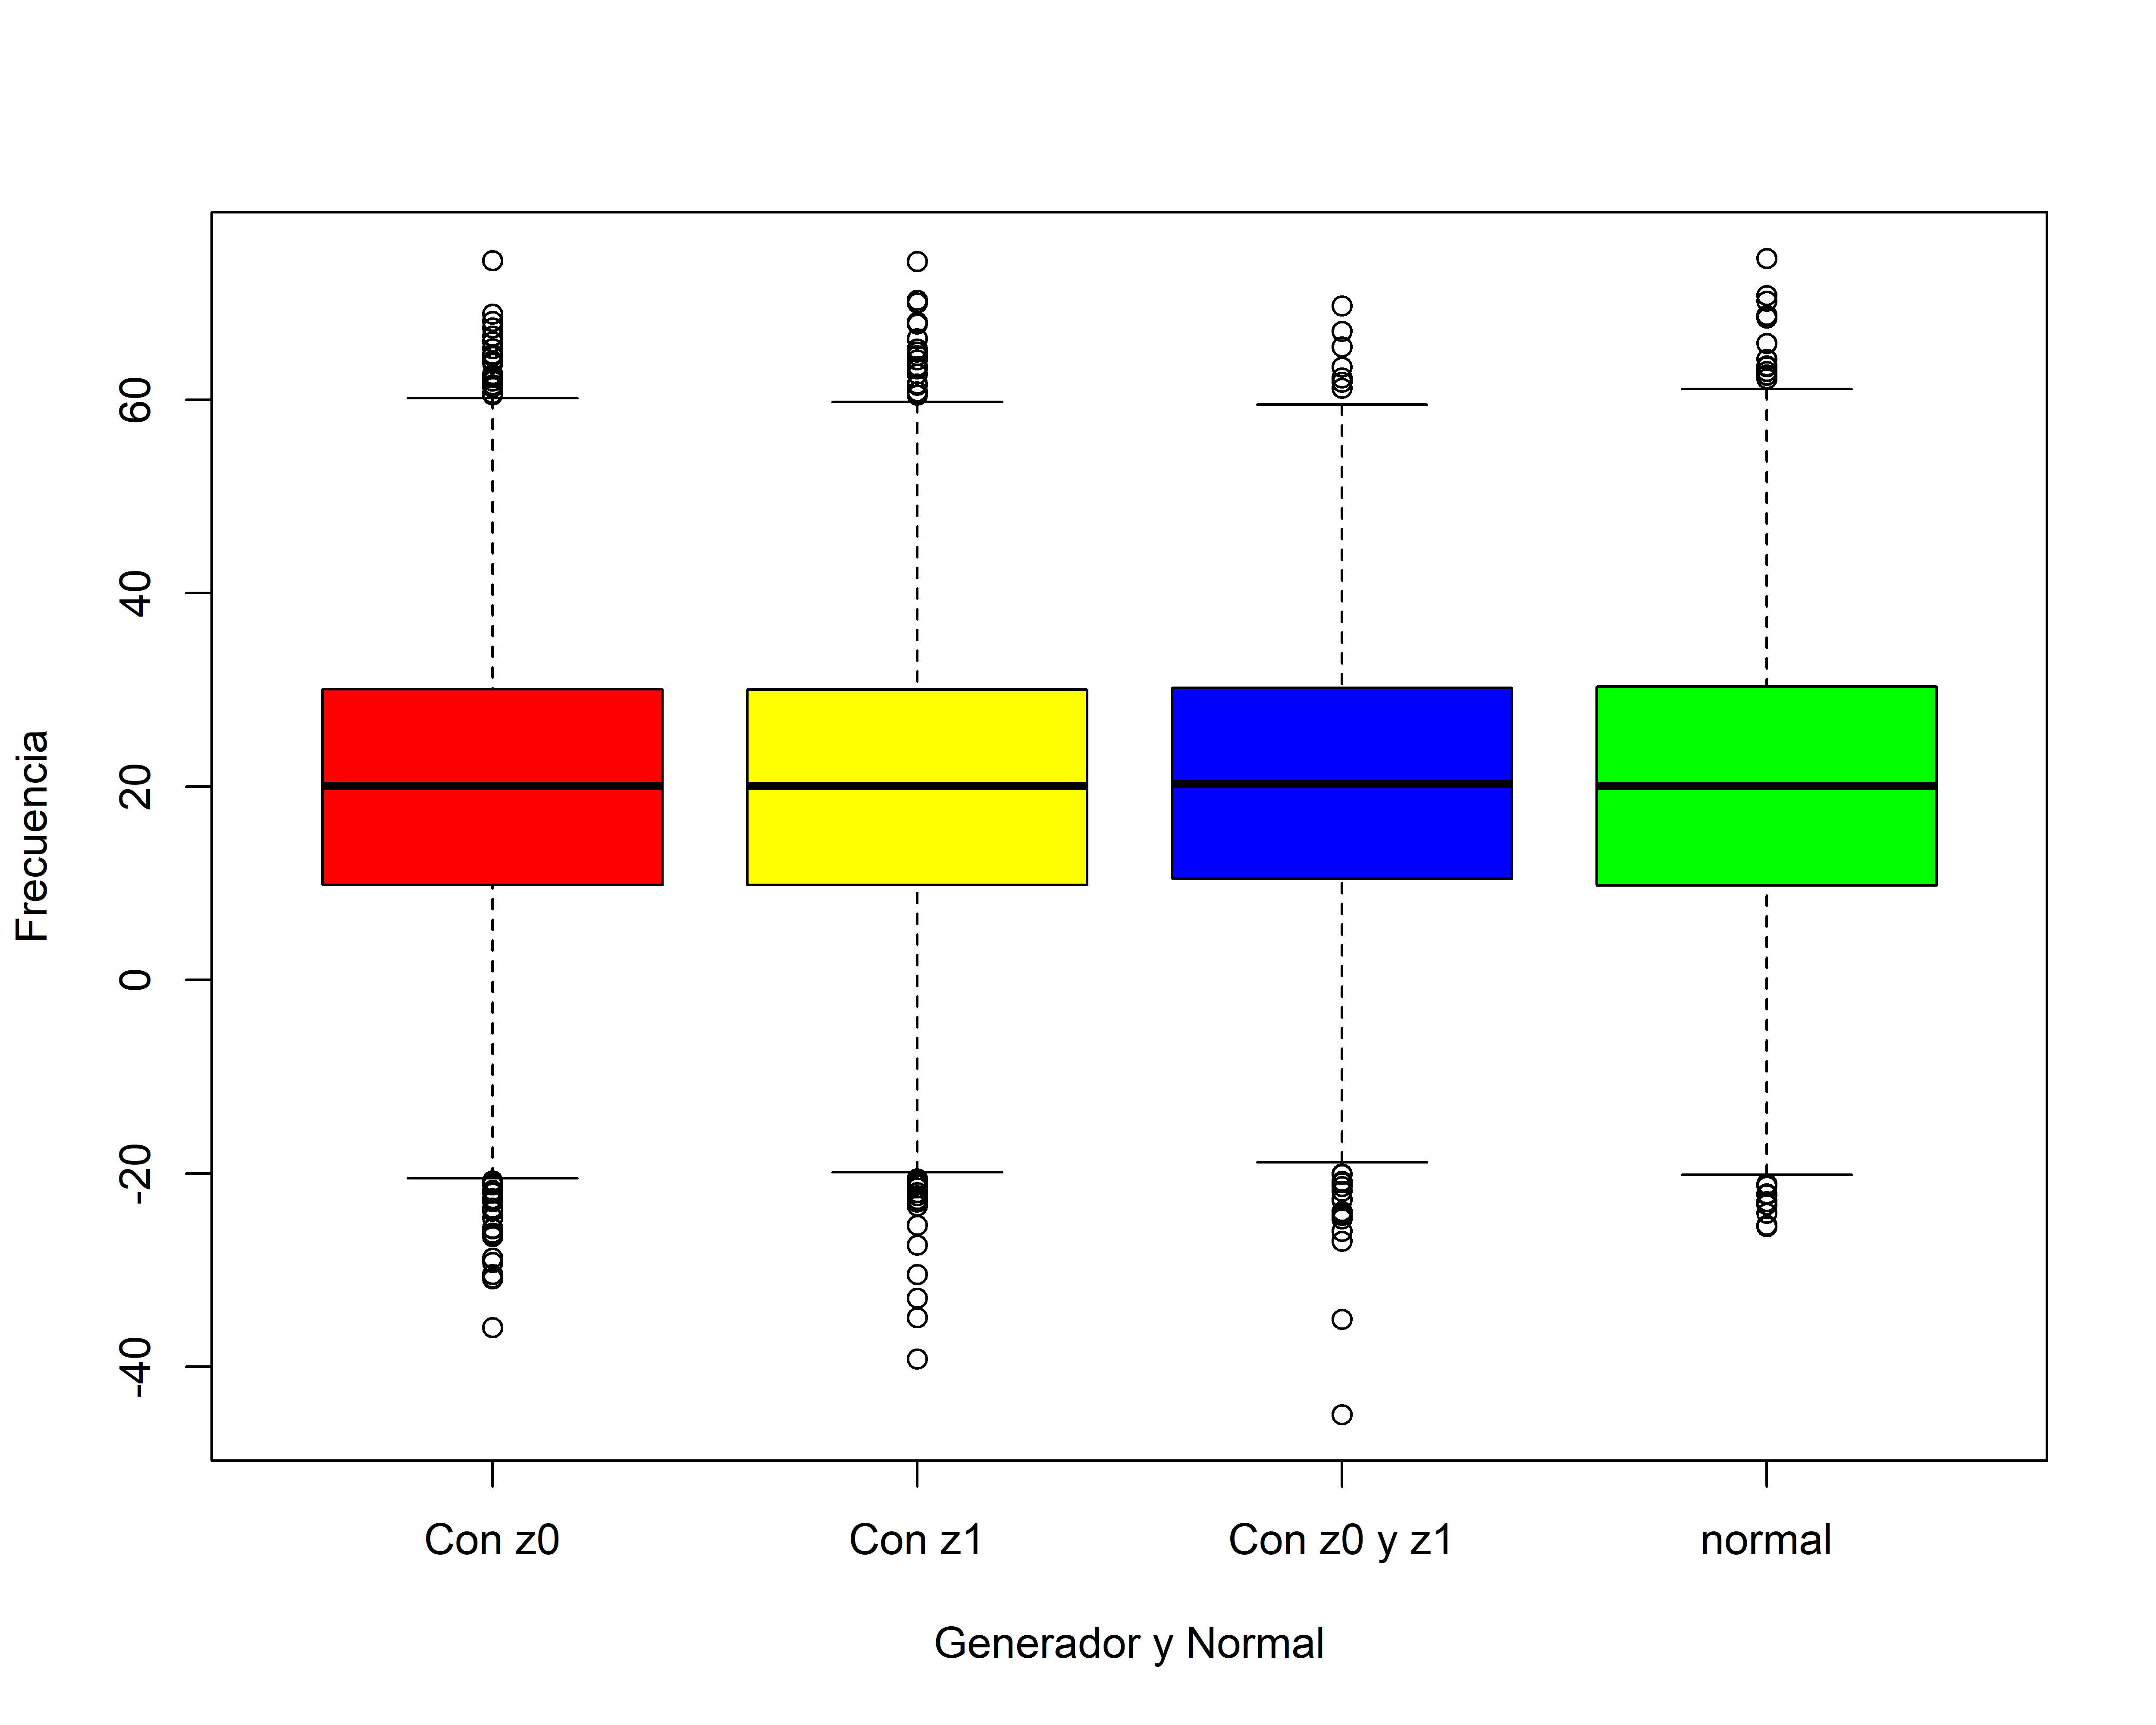
\includegraphics[width=\linewidth]{Figures/comparativosZ.png}
\caption{Comparación de diagramas de caja y bigotes del generador considerando sólo $z_{0}$ (rojo), con sólo $z_{1}$ (amarillo), ambas variables $z_{0}$ y $z_{1}$ (azul) y los resultados obtenidos por la función \texttt{rnorm} (verde), con $n= 4,500$ replicas, media ($\mu = 20$) y desviación estándar ($\sigma = 15$)}
\label{escenario2-3}
\end{figure}

\subsection{Uso del generador de números pseudoaleatorios con distribución uniforme en el generador de números pseudoaleatorios con distribución normal}

A manera de práctica, se utiliza el generador de números pseudoaleatorios con distribución normal, modificando el algoritmo \ref{boxmuller}, de tal manera que las variables $U_{1}$ y $U_{2}$ se obtienen a partir del generador de números pseudoaleatorios con distribución uniforme tratado en la sección \ref{distuniforme}. 

Para llevar a cabo la experimentación, se consideran los siguientes parámetros para el generador de distribución uniforme: $X_{0}=21$, $a = 8,001$, $c = 2,651$ y $m = 2,048$ con $n=2$ réplicas y para el generador para los de distribución normal, $n= 4,500$ replicas, media ($\mu = 20$) y desviación estándar ($\sigma = 15$). Los resultados obtenidos de esta experimentación son mostrados en la figura \ref{uniformeNormal}. En la que podemos observar que los datos obtenidos con el generador se ajustan a una la distribución normal y, por lo tanto, el generador de números pseudoaleatorios con distribución uniforme, está arrojando valores con está distribución.

\begin{figure}
\centering
\includegraphics[width=\linewidth]{Figures/uniformeNormal1.png}
\caption{Correlación entre los valores obtenidos del generador (transformación de Box-Muller) y la distribución normal, con $n= 4,500$ replicas, media ($\mu = 20$) y desviación estándar ($\sigma = 15$)}
\label{uniformeNormal}
\end{figure}


\bibliography{refProbabilidad}
\bibliographystyle{plain}

\end{document}

